\section{ХОД РАБОТЫ}

\subsection{Постановка задачи}

В ремонтную службу предприятия поступают средства для наладки. Интервалы между
моментами поступления инструментов составляют от $10$ до $20$ минут.

Сначала все инструменты поступают к одному из трёх наладчиков. Наладчик выполняет
их мелкую наладку и (при необходимости) полную наладку. Мелкая наладка
требуется для всех инструментов и занимает ровно $10$ минут. Полная наладка
требуется примерно для $60\%$ инструментов; она занимает от $20$ до $40$ минут.

Для всех инструментов требуется проверка на стенде автоматического контроля.
Для инструментов, для которых выполнялась только мелкая наладка, такая проверка
занимает от $5$ до $10$ минут. Для инструментов, для которых выполнялась
полная наладка, проверка занимает $15$ минут.

Затраты, связанные с мелкой наладкой инструмента, составляю $3$~ден.~ед., затраты
на полную наладку --- $8$~ден.~ед., на проверку на стенде --- $5$~ден.~ед.

Требуется разработать GPSS-модель, имитирующую работу ремонтной службы в течение
$100$ часов. Программа должна сообщить:

\begin{itemize}
  \item количество инструментов, для которых потребовалась только мелкая наладка;
  \item количество инструментов, для которых потребовалась полная наладка;
  \item общие затраты на наладку всех инструментов.
\end{itemize}

\subsection{Решение задачи}

Разработанная GPSS-модель представлена в приложении~А. После выполнения сеанса
моделирования исходной задачи, получим отчёт, представленные на
рисунках~\ref{pic:report_1}~-~\ref{pic:report_3}.

\begin{figure}[h!]
  \centering
  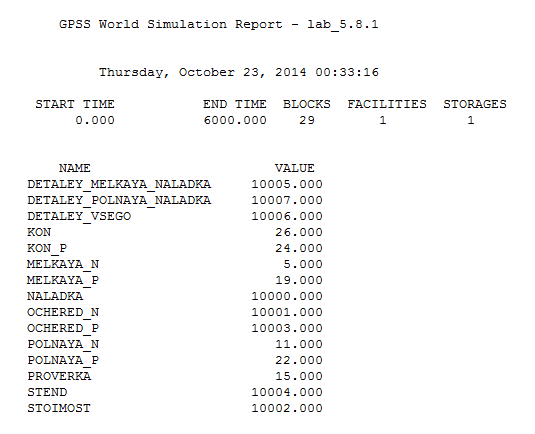
\includegraphics[width=0.75\linewidth]{pic/report_1}
  \caption{Выходные данные имитационной модели}
  \label{pic:report_1}
\end{figure}

\begin{figure}[h!]
  \centering
  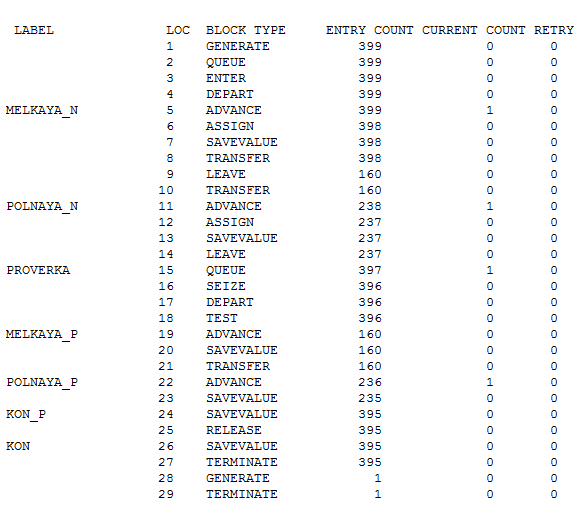
\includegraphics[width=0.75\linewidth]{pic/report_2}
  \caption{Статистика исполнения команд имитационной модели}
  \label{pic:report_2}
\end{figure}

\newpage

\begin{figure}[h!]
  \centering
  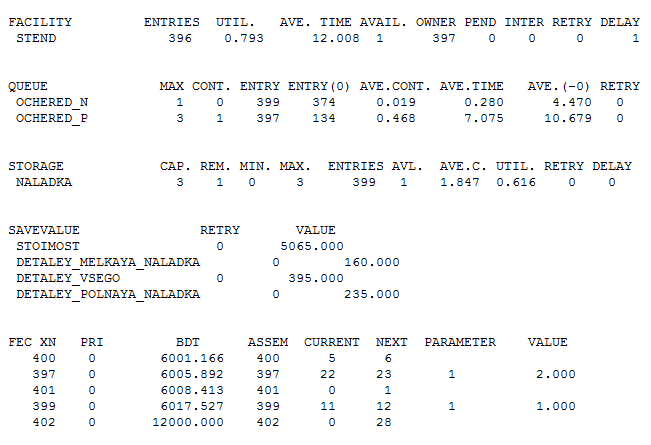
\includegraphics[width=0.9\linewidth]{pic/report_3}
  \caption{Статистика использования узлов имитируемой СМО}
  \label{pic:report_3}
\end{figure}

Из рисунка~\ref{pic:report_3} видно, что в процессе работы программы были
получены значения, предложенные ранее к отысканию:

\begin{itemize}
  \item количество инструментов, прошедших мелкую наладку --- $ 160 $;
  \item количество инструментов, прошедших полную наладку --- $ 235 $;
  \item общее количество инструментов --- $ 395 $;
  \item общие затраты на наладку всех инструментов --- $ 5065{,}0 $.
\end{itemize}

\newpage
